\newpage
\section{Экспериментальная часть}

Необходимо протестировать написанную программу.

\subsection{Примеры работы}

Примеры работы программы представлены на рисунках
\ref{img:zero_arg}, \ref{img:good}, \ref{img:not_found}.

\begin{figure}[H]
    \centering
    
\includegraphics[scale=0.4]{zero_arg}
    \caption{Пример работы без аргументов}
    \label{img:zero_arg}
\end{figure}

\begin{figure}[H]
    \centering
    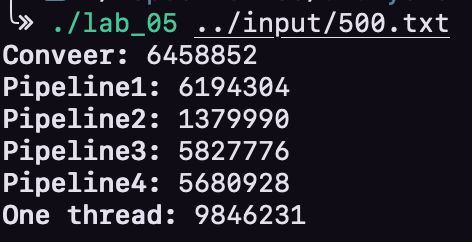
\includegraphics[scale=0.8]{good}
    \caption{Пример работы с найденной подстрокой}
    \label{img:good}
\end{figure}

\begin{figure}[H]
    \centering
    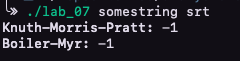
\includegraphics[scale=0.8]{not_found}
    \caption{Пример работы без подстроки}
    \label{img:not_found}
\end{figure}

\subsection{Результаты тестирования}

Результаты тестирования представлены на таблице \ref{table:test_result}.

\begin{table}[H]
    \caption{Результаты}
    \label{table:test_result}
    \centering
    \begin{tabular}{|c|c||c|c|}
        \hline
        Строка & Подстрока & Результат работы КМП & Результат работы БМ \\
        \hline
        \hline
        abababbc & ababbc & 2 & 2\\
        \hline
        qwe & qwe & 0 & 0\\
        \hline
        asdasd & sa & -1 & -1 \\
        \hline
        abababa & baba & 1 & 1 \\
        \hline
    \end{tabular}
\end{table}

Все тесты пройдены успешно.

\subsection{Выводы}

Написанная программа прошла все тесты успешно.
